%# -*- coding:utf-8 -*-
%!TEX root = ../thesis.tex
%%==================================================
%% chapter01.tex for SJTU Master Thesis
%%==================================================




\chapter{绪论}
\label{chap:Introduction}
% 1.1 研究背景及意义
% 1.2 水下机器人系统描述
% 1.3 水下机器人的控制特性以及研究进展
% 1.4 本文主要研究内容
% 1.4 本文的主要创新点
\section{研究背景及意义 }

地球表面积三分之二以上都是海洋,近三分之一以上的人类生活在近海和近河流湖泊地带。随着陆地水资源的不断消耗,对蕴含丰富生物资源与矿产资源的海洋的开发成为了人类生存与发展所关注的一个新的重要领域\cite{fossen1994guidance,Fossen2002Marine}。目前,世界各国愈发关注海洋探索,而作为其中探索率较低的水下世界,近年来越来越受到国家、企业等各种力量的关注,探索并开拓水下世界成为了国家、企业投资发展的一个重要战略组成\cite{bottaccini1954stablity,John1978Methods}。

\begin{figure}
\centering
\includegraphics[width=9cm]{figure/chap1/seadragon.jpg}
%\captionsetup{justification=centering}
\label{fig:chap1:F1}
\bicaption[fig:chap1:F1]{深海作业ROV-海龙 III}{深海作业ROV-海龙 III}{Fig.}{SeaDragon III ROV for observation}
\end{figure}

\begin{figure}
\centering
\subfigure[水下滑翔机]{
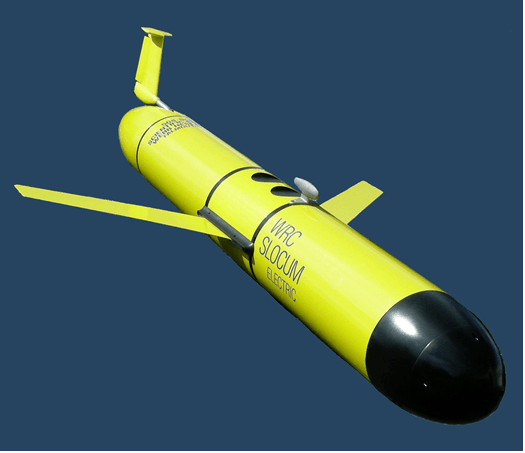
\includegraphics[width=6cm, height = 6cm]{figure/chap1/glider.png}}
\subfigure[REMUS 600型AUV]{
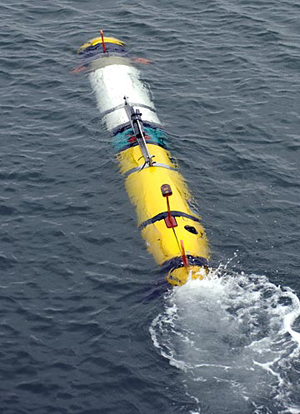
\includegraphics[width=6cm, height = 6cm]{figure/chap1/remus600.jpg}}
%\captionsetup{justification=centering}
\label{fig:chap1:F2}
\bicaption[fig:chap1:F2]{非缆控型水下航行器}{非缆控型水下航行器}{Fig.}{Underwater vehicle without cable}
\end{figure}

由于海洋环境与人类生存的陆地环境存在较大的差异,人类的科研与生产活动不能直接在水下实现。因此人类在探索、认识水下环境以及利用海洋中的资源主要借助于多种不同类型的水面、水下探测与作业设备来实现目标(如图\ref{fig:chap1:F1},图\ref{fig:chap1:F2}和图\ref{fig:chap1:F3}),其中图\ref{fig:chap1:F3}给出水下机器人贴近侧壁进行航行观测)\cite{oien2016dynamic,knausgaard2013development,drozdik2015dynamic}。水下机器人是一种目前世界上通用的一种较为先进的水下航行系统,其主要用于帮助人类对水下环境、结构物、海底管道以及其他水下设备进行观测和辅助作业\cite{fossen1994guidance,Fossen2002Marine,berg2012development,drozdik2015dynamic,feng2005intros}。水下机器人,又称水下航行器,主要由推进动力系统、能源管理系统、控制与通信系统和机械本体组成,其动力和控制可以由水面站进行供给和设置,也可由水下机器人本体压力舱内的便携电源管理系统和自动导航仪进行供电和运动导航\cite{fossen1994guidance}。

\begin{figure}
\centering
\subfigure[BLUEROV模型]{
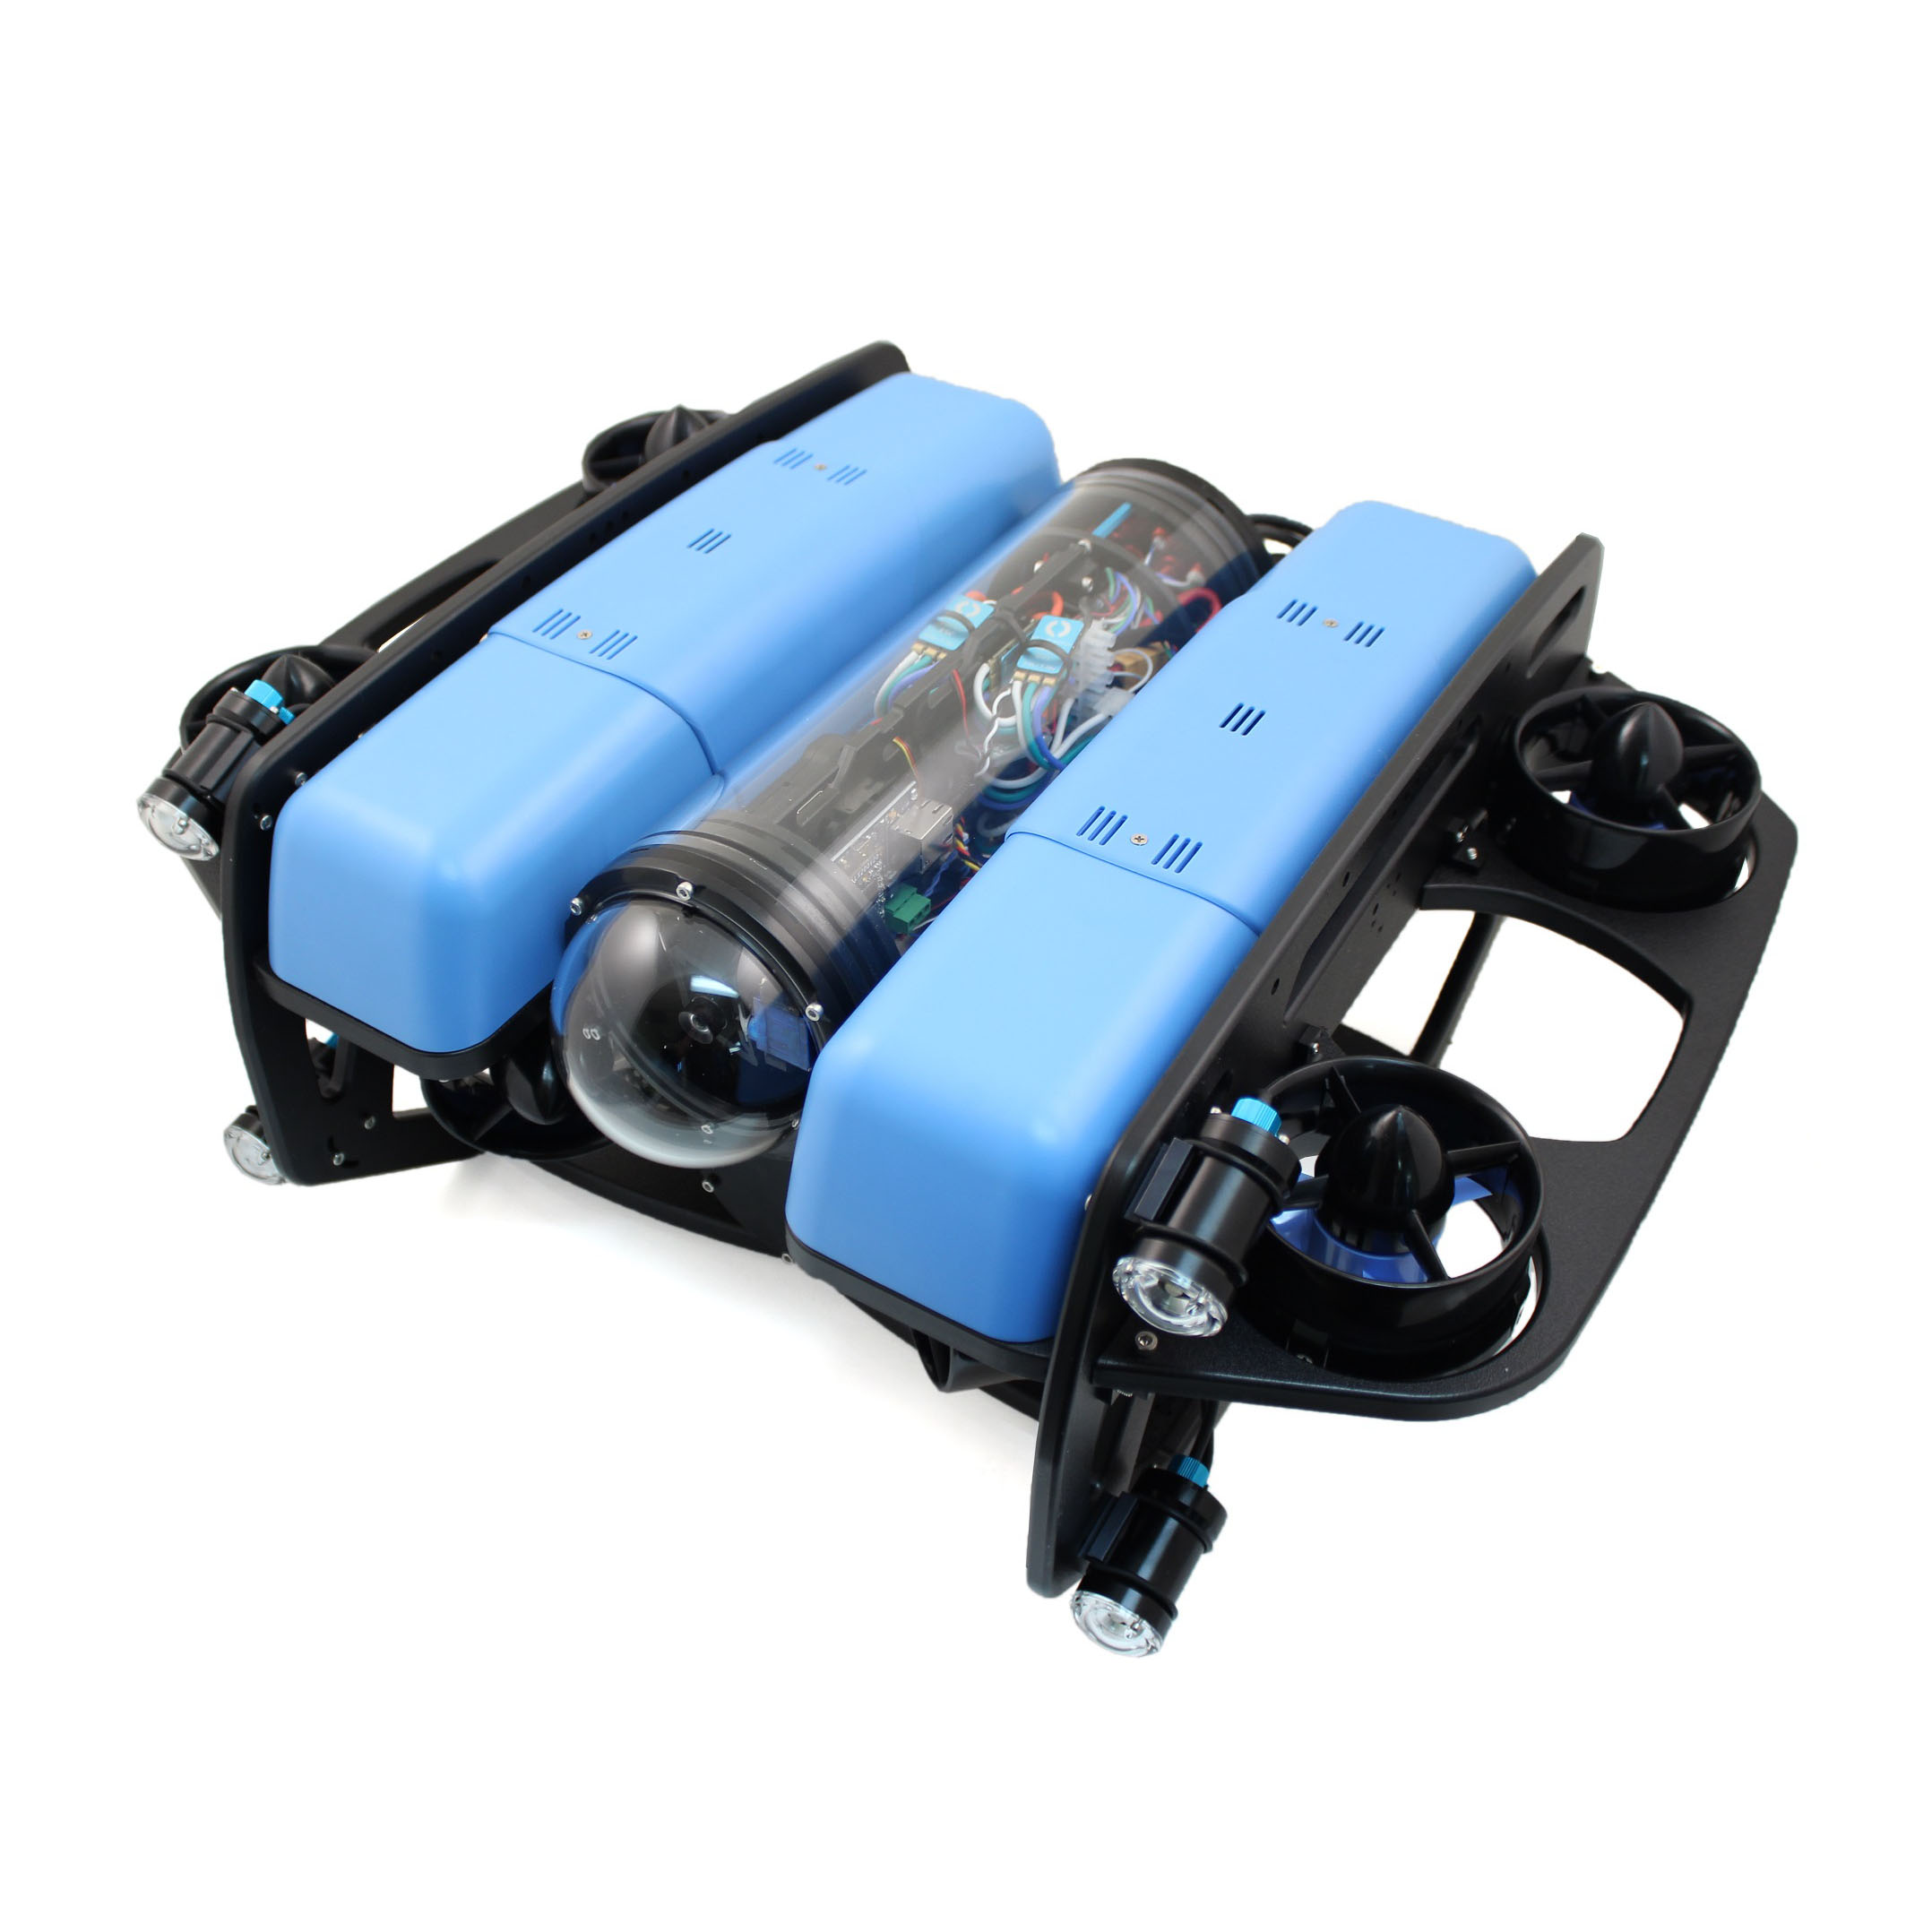
\includegraphics[width=6cm, height = 6cm]{figure/chap1/heavybluerov.jpg}
}
\subfigure[贴近侧壁观测]{
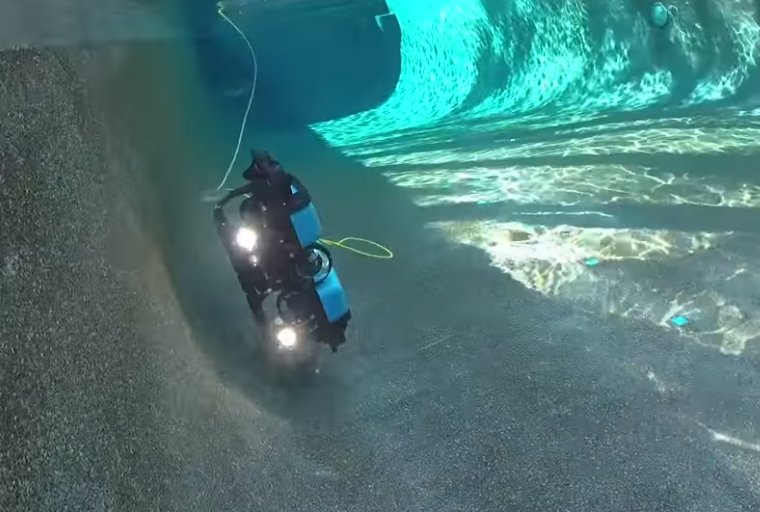
\includegraphics[width=8cm, height = 6cm]{figure/chap1/heavyblue.png}
}
%\captionsetup{justification=centering}
\label{fig:chap1:F3}
\bicaption[fig:chap1:F3]{小型缆控水下机器人BLUEROV}{小型缆控水下机器人BLUEROV}{Fig.}{Small ROV named BLUEROV}
\end{figure}


水下机器人根据控制方式不同,可以分为自治水下机器人(AUV)和有缆遥控水下机器人(ROV)。其中,由于带缆遥控潜水器(ROV)有着能在未知甚至危险的水下环境中完成长时间且相对可控的高强度、多形式的作业与观察的优异性能,因此ROV被广泛地应用在海洋水下环境的探索与开发活动中。ROV的应用主要集中在如下几个方面:海洋资源调查、海底海床绘制、海洋管道检测、水下矿物质或生物样本采样、以及未知水下领域的目标观测等\cite{follestad2017autonomous,aguiar2007dynamic}。AUV型水下航行器有着很强的自主性,能够到达的水下区域更加广阔,其主要用于海洋水质监测、水下资源探索、水生物观测、军事、水下传感器网络数据收发等\cite{maalouf2013contribution}。目前,水下机器人的探索开发应用有不断走向深海和远海的自主化趋势,为水下机器人的相关建模与控制技术带来了挑战\cite{wangbiao2016,yangke2014,yangrui2015,aakre2016development}。并且,由于水下机器人工作的水下环境具有高度复杂和强时变性,再加之水下机器人系统本身可能会因环境变化而产生不确定性,这些都会对水下机器人系统的运动稳定性与可靠性带来影响。因此,搜索并建立精准的水下机器人模型以及设计出考虑水下机器人非线性的鲁棒自适应控制的研究越来越受到国内外的学者关注\cite{yang2014modeling,haugen2012modeling,knausgaard2013development,eidsvik2015identification,eng2014added}。此外,水下机器人也可以基于动力学系统的控制输入个数与系统自由度的关系,研究不同动力布置的水下机器人的控制与动态系统的瞬态优化\cite{fantoni2002non,russdrakebook}。自然界中很多动态系统存在一些自由度没有控制输入,机器鱼、机器鸟虽然被设计开发出来,但是表现出来的性能与自然界所参考的生物本身相比,运动总是那么的不自然\cite{russdrakebook}。水下机器人的运动是通过设计状态反馈控制器来实现的,虽然可以达到控制目标,但是设计的运动大多忽略了系统本身的动态,例如系统中的非线性\cite{russdrakebook,galeani2009tutorial}。

水下机器人相关技术的研究如何,关系到水下机器人是否能够成功被应用于水下勘测、水下辅助作业、任务规划\cite{Souza2007Intelligent}。如何提高水下机器人的水下运动与导航性能的问题本身涉及的因素很多,其中对提高水下机器人系统整体性能起着关键作用的问题主要有水下机器人与环境模型的建立与识别、提高控制器对于模型非线性特性的自适应性与鲁棒性、考虑水下机器人设备所具有的驱动器非线性\cite{yang2012observer,sarhadi2016adaptive2}。水下机器人的模型用来解释本体运动与施加在本体上的力、力矩之间的关系,该模型对于控制和导航都具有重要作用\cite{wu2016parametric}。模型经常被用来观察水下机器人系统的状态,而因此水下机器人模型的准确性就很重要。水下机器人模型建立不仅仅是为了分析,也要更方便研究者和系统设计者的控制器设计工作。基于运动学和动力学的有关知识建立的水下机器人动力学模型是基于以往历史的理论认识,这种认识具有一定的指导性,但也具有一定的偏见性\cite{menezes2014symbolic}。水下机器人的模型包括数学模型的公式形式与具体模型参数\cite{schmidt2009distilling}。以往的系统辨识方法是基于确定的模型结构采用最小二乘法、遗传算法等优化搜索方法来辨识具体的模型参数,这种方法在模型结构确定的情况下具有较好的适用性与可靠性,但是机器人的动态系统从时间过程演化的角度来看,水下机器人的模型是否结构一直保持不变\cite{John1978Methods}?水下机器人进行系统参数辨识时,辨识的目标函数也是基于某种特定条件下的理论而得到的,随着水下机器人的运动不断进入到未知的区域,系统辨识的模型就可能会失去价值。系统辨识的前提一般是模型结构一定,然而没有一种方法能够自动地获取水下机器人模型的数学结构与参数\cite{wu2016parametric}。

对于被完全理解的系统所建立的模型可以很好的描述系统状态,然而水下机器人系统的非线性以及环境的未知性会对系统的搜索与确定带来困难。为了解决这一问题,启发式建模方法例如符号回归方法被用来搜索并确定水下机器人模型的映射关系与模型参数。由于用于进行模型参数学习和搜索的经验数据是在一定的实验条件下获取的,该数据获取方法的人力代价和实验成本都很高昂,且从成本上更加不适用于复杂形状的大型水下机器人(如图\ref{fig:chap1:F1})\cite{yang2014modeling}。为了快速而准确地获取水下机器人用于控制的模型,参数辨识、模型简化以及数值建模技术被用于本文的研究。由于水下机器人的运动具有高度非线性并且受到不确定性的扰动影响,在设计水下机器人的控制器时,需要给线性动态系统中添加不确定性和未建模动态\cite{valladarez2015adaptive}。水下机器人的控制器设计时要保证两个原则:鲁棒性和自适应。鲁棒性可以保证水下机器人系统在意外最坏情况出现时而不失效,自适应性可以保证水下机器人系统可以更好地适应环境中的不确定性与干扰。水下机器人动态系统的非线性包括一般非线性(模型参数时变、模型结构变化)和特殊非线性(驱动器阈值、死区特性)\cite{Wu2018Pitch}。鲁棒自适应控制虽然是为了解决模型的不确定性而设计,但是它不是所有问题的万能解决方案\cite{lavretsky2013robust}。因此,为了确保水下机器人的工作性能,在设计水下机器人的控制器是需要考虑水下机器人的驱动器的非线性特点,使用现代补偿器控制策略来对自适应控器进行优化,以保证水下机器人的控制性能。

综上所述,本文研究搜索水下机器人的数学结构与模型参数、建立用于控制机制的水下机器人模型并设计带有输入饱和补偿特性的鲁棒自适应控制器,可为水下机器人系统的智能应用提供参考。

% \section{水下机器人系统研究现状  }

\section{水下机器人系统建模研究现状 }

本研究分别从运动动力学理论建模和数据驱动的建模两个角度展开,主要包括水下机器人的运动动力学建模与关键项计算、基于实验数据的数学模型的结构表达搜索与参数辨识以及水下机器人对于环境水流的感知。水下机器人的空间运动建模主要有两种方法:一是根据推进器推力布置,基于牛顿运动定律进行的建模,其中有阻尼、附加质量等;第二种方法是采用系统辨识方法对获得的实验数据进行参数辨识,根据选择的模型结构与公式,确定相关水动力参数;第三则是水下机器人的建模是有其应用目标的,基于控制应用的导向,采用数值计算方法与模型简化获得用于非线性自适应控制的方程。

\subsection{水下机器人的动力学运动学建模  }

通过对水下机器人进行运动与动力学分析,国外学者Fossen 系统地给出了AUV和ROV类型的水下航行器的流体动力学模型\cite{fossen1994guidance}。我国学者施生达、元泉等也基于潜艇理论可以将水下机器人的模型进一步划分为水平面模型和垂直面模型\cite{yuanchuan2001submarine,shishengda1995submarine}。

水下机器人形状和类型各异,这使得水下航行器的流体动力学模型中的各项所起的作用也会有所不同,在使用时应对水下机器人的模型进行一定的处理。根据水下航行器的类型与运行特点可提出一些假设,用于简化水下机器人的动力学模型\cite{Fossen2002Marine,fossen1994guidance,fossen2011handbook,yangke2014}。水下机器人模型虽然在使用的时候都会被简化处理,不过简化后的模型结构以及简化后用于求解模型参数的方法好坏仍然不同。AUV和ROV的简化模型现已经被广泛用于AUV、ROV的运动控制与导航规划中\cite{clement2016modeling,haugen2012modeling,prestero2001verification}。具体而言,在使用Fossen建立的运动动力学模型时,如何针对不同类型形状和应用目标的水下机器人进行流体动力学计算以确定模型中的参数成为一个富有意义却又实际的问题。为了整体地评估所设计的水下机器人的流体动力学性能,Evans在文中描述了自主水下航行器的动力学模型并使用流体力学计算方法评估了本体所受到的力以评估所设计的航行器的性能\cite{evans2004dynamics}。
水下机器人的外形不同,一般可以划分为流线型和复杂形状,因此不同航行器流体动力学性能计算的困难和速度也不同。而根据流体对本体作用的机理不同,研究者也分别从非初等几何复杂形状、附加质量、阻尼、流线型设计与性能角度展开了流体计算研究\cite{Wu2012Hydrodynamic,jones2002calculation,Tang2009Estimation,wan2017CFD,wang2001rovcfd}。Tang\cite{Tang2009Estimation}使用计算流体动力学用来估计具有复杂形状的水下机器人的流体动力学系数,并通过与实验结果对比验证计算所得的参数值。Wang\cite{wang2015numerical},Perrault\cite{perrault2003sensitivity}和Eng\cite{eng2014added}使用流体动力学软件(WAMIT)计算框架式ROV、 AUV的附加质量参数并通过实验验证计算的参数值的准确性。 Gibson\cite{gibson2015comparison}提供八个不同的流线型AUV模型,并使用最小二乘法和自适应辨识方法来近似估计阻尼模型的系数,通过对比,确定出哪个模型的线性阻尼性能更加优秀。

在运动动力学模型中,Garus\cite{garus2014thrust}介绍水下机器人的推进系统的推力分布方法,并根据运动要求和系统无故障的设定进行推力分布的优化,这对于理解设计水下机器人系统也很有益。本文中尝试建立了一种推力控制矢量用来表达每个推进器对整体控制的影响,以便于控制器的整体设计。此外,如何感知海洋运载器的环境要素在近年也受到研究者的关注\cite{muhammad2015flow,bouffanais2010hydrodynamic,tagliaferri2015wind}。设计小型水流侧线系统,并将系统装到水下机器人原型中,实验验证系统的可行性\cite{franosch2010biomimetic,abdulsadda2012artificial,yang2010artificial}。Jung\cite{jung2013flow}基于水下鱼类的侧线器官的水下环境感知机理,提出使用压力传感器网络来辅助控制,并使用二维平面运动分析流体动力学。本课题研究者针对鱼雷型UUV的不同的水流环境,基于鱼类侧线感知水流的机理,使用流体动力学模拟载体受到的水下情况,选择使用线性判别分析和支持向量机技术进行数据降维、训练以建立水流方向感知分类模型,从功能角度验证了仿生侧线感应水流的能力\cite{Wu2016lateralline,friedman2001elements}。
为了将水下机器人模型的建模工作与控制实践联系起来,Yang, Benoit和本课题作者对具有模型不确定性的水下机器人鲁棒控制的关键问题进行了研究\cite{yang2014modeling}。其中,在对具有复杂形状的AUV的模型建立进行研究时,开发准确的流体动力学模型受到高成本问题的制约,这为缩小模型的不确定性以提高控制的性能带来很大困难。该文作者使用流体计算软件对于低速AUV CISCREA进行面向控制的建模预测流体动力学关键参数:附加质量和阻尼矩阵\cite{yang2014modeling,yang2015modeling}。并且,在论文中研究者使用建立的模型进行$H_{\infty}$鲁棒控制方案设计,并用于偏航控制的实验验证\cite{yang2015modeling,yang2015robust,du2016robust}。


\subsection{数据驱动的系统建模 }

基于数据驱动的建模方法\cite{huang2015trends},目前主要是采用系统辨识,该方法需要确定所研究对象的数学表达结构,而近年来,研究者使用了多种方法进行非线性系统的辨识研究\cite{deng2009system}。Kim\cite{kim2012estimating}等人提出了一种无需模型的方法来估计自由飞行物体的动力学,使用非线性回归方法和局部投影回归方法,对乒乓球体运动进行实时跟踪估计,并使用EKF来增强估计模型的鲁棒性。Baruch\cite{baruch2009levenberg}提出一种新型的循环神经网络模型用于系统辨识, 并使用反向传播 和递归Levenberg-marquart算法用于估计自适应控制的状态。Feng\cite{feng2006identification}为解决岩石的应力非线性表达问题,提出一种改进的粒子群优化的遗传算法对岩石的材料模型结构和相关参数进行系统识别,该方法可以同时识别模型的结构和参数。在海洋运载器的研究上也有大量的研究者从事探索\cite{luque2011auv,hegrenaes2007comparison,hong2013online},其中Sabet\cite{sabet2014extended}提出了一种用于估计水下机器人的流体动力学系数的方法,分别使用了扩展卡尔曼滤波和无迹变换卡尔曼滤波方法来辨识具有强非线性的水下机器人的模型的参数,结果发现UKF要优于EKF。Wang\cite{wang2014sensitivity}与Xu\cite{xu2013identification}分别使用4自由度的船舶操纵数学模型和6自由度运动模型获得实验数据,通过分析数据,使用SVM回归方法确定模型中的流体力学系数,通过将预测结果与实际对比,以证明方法的有效性。
其中,来源生物进化的遗传算法也被用于研究非线性系统辨识问题,Zhou提出基于遗传算法的时域识别算法,通过将遗传算法(GA)应用于分阶系统的识别\cite{zhou2013genetic}。Chang提出一种应用于非线性系统的识别和控制的遗传算法,尝试使用实际编码来描述系统,假定结构的情况下,估计系统模型\cite{chang2007nonlinear}。为了更好的将系统辨识的目标方程在生物进化中更好地表达,Santos采用基因编程(GP)方法的树状结构被用来描述识别问题,并使用该方法辨识提升阀的进气口与排气口的数学关系,将GP方法用于系统识别的结构选择问题,通过自动修改基因表达树的结构和组成,以此来辨识非线性的球管系统\cite{dos2014genetic,dos2009nonlinear,Mcconaghy2008Genetic}。Gandomi提出一种新的方法,使用多基因遗传规划方法来研究经典回归辨识中的非线性模型的互相作用问题,并在复杂的结构工程问题中进行实例验证说明\cite{Gandomi2012A1,Gandomi2012A2}。
虽然系统辨识可以用来确定非线性模型的系数,但是它的研究会基于一个前提,即已知的数据表达的假设,所限制,这对于人类进行快速有效的自动建模是一种阻碍\cite{menezes2014symbolic}。符号回归是一种回归分析,它从精确度和结构演化两个方面搜索数学表达式的空间,以找到最适合给定数据集的模型,该方法并没有提供特定的模型作为算法的起点。相反,通过随机组合数学建模功能块(例如数学运算符,分析函数,常数和状态变量)来形成初始表达式,然后通过使用遗传编程重组前述方程形成新方程\cite{schmidt2009distilling,wu2016parametric}。
受自然启发的机器学习技术如符号回归方法、稀疏回归等启发式搜索方法被用来从经验数据中自动学习模型用于研究复杂的网络现象\cite{menezes2014symbolic,brunton2016discovering}。为解决寻找自然规律和数学方程的过程不能自动化的问题,Schmidt提出一个确定非重要性原则,并通过从数据集中自动搜索运动方程以验证所提出算法的有效性\cite{schmidt2009distilling,schmidt2010symbolic}。Schwab提出一个灵活的知识表示框架,它利用符号回归学习和数学表达式来从数据中获取规律,该算法可以通过挖掘数据以产生新的规律描述,并添加到知识库中用来提高整体的学习性能\cite{schwab2012learn}。
由于不要求指定特定模型,符号回归不受人类偏见或领域知识中的未知空白的影响。它试图揭示数据集的内在关系,通过让数据中的模式本身揭示适当的模型,而不是强加从人类视角在数学上易于处理的模型结构。这有助于推理,并有利于获得有关数据,以生成对系统的洞察。Eureqa软件从数据中生成清晰的数学表达式,并根据表达式结构是否已知,可以分别搜索模型的数学结构和精确地拟合出模型,进而可以计算模型的参数\cite{stoutemyer2013can}。在对水下机器人的建模中为了更好了解实际运动中的各个变量的数据集的映射关系,本课题的研究者使用实验数据,选择使用基于自然选择的符号回归方法,自动地检测水下机器人本体的数学结构,并且所提出的方法也可以用来辨识模型参数,且性能经过与Levenberg-Marquardt算法和遗传算法对比,以验证提出的方法的有效性\cite{wu2016parametric,Moreno2015Symbolic}。


\section{非线性自适应控制现状 与水下机器人控制特性 }

自适应控制律和参数更新律往往是直接基于线性的无干扰、无噪声、无未建模动态的动态系统来设计的,这种控制方法容易开发,但是在实际应用中会与实际系统的模型不一致而给控制带来偏差。一个受控制系统如果因为系统是非线性的,它的参考模型是低维度的,且实际控制的系统是高维度的\cite{russdrakebook}。控制参考模型系统与实际系统之间的偏差会影响水下机器人系统的稳定性与运载器的轨迹追踪性能\cite{li2005design,jun2009development,garcia2014modelling,wang2016fast}。为了更好地设计出适用于实际系统的控制器,水下机器人的控制系统必须要靠非线性、未建模干扰、有界噪声等因素,并使用接近于现实的复杂非线性全自由度模型系统进行验证。

非线性自适应控制的具体设计主要是控制器的设计考虑了模型的多种不确定性以及有界的干扰。有些自适应控制器在存在小干扰的情况下会变得不稳定,出现参数漂移问题。这非常的糟糕,也曾在学术界引起的了讨论。许多人员从自适应控制器的设计的多种角度进行分析和研究,试图找到自适应控制器的不稳定的原因以及消除不稳定的方法。设计出稳定的自适应控制方法并可适用于实际系统的指令跟踪,即产生了鲁棒自适应控制的设计方法。鲁棒自适应控制的目的是为了解决动态系统中存在的模型不确定性和扰动,Lavretsky 和 Ioannou 试图从多个不同的角度来分析不稳定机制,并对存在的自适应控制方法进行修改,以期得到可以适用于广泛动态系统的自适应控制方法,并最终在实际系统中应用此方法,如飞机\cite{lavretsky2013robust,Ioannou2012}。

在水下机器人系统的控制设计中,首先是要获得准确的航行器系统描述。然而,实际的海洋机器人系统因为工作的水下环境的复杂多变而具有较大的不确定性。水下机器人的建模需提供准确的模型用于设计,这样的模型既要能够表征系统的主要运动特征又不能太过复杂,使得控制器的设计变得异常困难\cite{fossen1991nonlinear,beinset2007controller,eriksen2015horizontal}。过度简单的模型虽然容易控制但是寻求控制器最优解的过程会变得过于漫长,又或者设计的控制器的调参要耗费很大的精力\cite{sutton1998reinforcement,madady2008pid}。本文的研究尝试使用鲁棒自适应控制的基础方法来分析水下机器人的位姿控制问题,根据鲁棒控制器中具体模块部分的设计要求的不同,分别对参考模型的更新与动态更新,自适应律的计算稳定性与速度以及水下机器人的系统非线性特征进行研究。


\subsection{鲁棒自适应控制的研究进展  }


鲁棒控制可看作一种在线控制策略,它能对可能包含有界不确定性的系统进行调节校正,该方法往往利用反馈-前馈状态输出关系产生相应的控制输入,从而使设备输出沿预定的“轨迹”变化,自适应控制对过程不确定性进行在线估计,然后产生控制输入以预测、克服或者尽量减少相对于预期闭环设备行为的不利偏差,可以将自适应控制看作是线性反馈积分器的非线性拓展\cite{lavretsky2013robust}。大多数的实际系统中,纯粹的鲁棒控制或者是自适应控制都不能做到更好的效果,因为系统总会有不确定性和非线性情况,而将两者结合是一种有益的尝试,也得到了诸多研究者的关注。

基于传统的模型参考自适应框架,Lavretsky系统性地研究鲁棒自适应控制,其中状态反馈直接模型参考自适应控制和具有积分反馈的模型参考自适应控制方法在航行器上的应用具有实用意义,并且为了抑制有界扰动,可以使用射影理论对模型参考自适应控制(MRAC)进行设计\cite{lavretsky2013robust}。Lavretsky基于预测器进行模型参考自适应控制设计,并将其与传统的模型参考自适应控制进行对比,仿真验证所提出的控制器能改进瞬态特性\cite{lavretsky2010predictor}。 在航空航天应用中,鲁棒自适应控制也得到了实践验证\cite{gregory2010flight,hyde2011flight}。 在低成本的四旋翼飞行器上,模型参考自适应控制用于对线性控制器进行增广,并且使用Lyapunov稳定性理论证明控制器的稳定性,该方法可以应对推力损失带来的不确定性\cite{Dydek2015Adaptive}。 基于模型参考的自适应控制响应特性也得到关注,射影理论被用于改善自适应的瞬态性能\cite{gibson2012improved}。 Gibson对闭环系统的直接和间接模型参考自适应控制的鲁棒性、稳定性以及瞬态性能进行了分析\cite{gibson2012adaptive} 。此外,随着技术发展,柔性飞行器的控制问题也采用自适应方法用于解决本体的挠度问题\cite{gadient2012very}。这些研究表明了自适应控制对于解决科研中热点问题的潜力。

基于MRAC架构的鲁棒自适应控制被用于非线性系统的控制,并且与不同的控制架构的非线性自适应控制性能也进行了对比\cite{kharisov2010comparison,kharisov2014comparison}。相比于MRAC框架,$L_{1}$自适应控制(L1AC)作为一种新的控制理论在瞬态性能、自适应估计不确定性和干扰、稳定性都被进行了理论证明\cite{Cao2006Design,cao2008adaptive,cao2010stability,wang2011l1,Hovakimyan2008adaptive}。此外,Hovakimyan在著作中全面阐述了开发的L1AC的控制理论,该方法的关键特点就在于将适应性与鲁棒性解耦,以提高自适应控制器的瞬态性能和鲁棒性\cite{hovakimyan2010L1}。Cao提出一种新颖的自适应控制框架,该框架下确保了控制器的输入输出两个信号的同时有界瞬态性能,其中该控制依靠低通滤波器与小增益定理来证明控制架构的稳定性,并对自适应控制最重要的非线性和模型不确定性都进行解决\cite{cao2010design,Cao2006Design1,Cao2006Design2,Cheng2008L1,Cao2008L1}。而在实践中,Kaminer通过设计一种三维空间的路径跟踪算法并使用商用的飞控将L1AC控制从理论带入实践中,验证了L1AC框架的优越性\cite{Kaminer2010Path}。Holhjem,Leman分别研究了F16和X-48B飞机在存在明显耦合的动力学和控制的纵倾和控制面失效下的L1AC控制实践\cite{holhjem2012l1,leman2010l1}。Dobrokhodov实施$L_{1}$自适应控制器在飞控上的故障恢复\cite{dobrokhodov2008flight}。NASA AirSTAR\cite{gregory2009l1}、空中加油\cite{wang2009l1,Wise2008Verifiable}、超音速飞机\cite{Lei2007Design}、油井钻进系统\cite{Zhiyuan2009Integrated}以及多种航行控制器系统的设计与验证\cite{dobrokhodov2008flight,wang2008l1,aguiar2008time,kharisov2008l1}中均采用$L_{1}$自适应控制解决问题。这些都证明了L1AC控制框架的优越性。

而在海洋机器人上,自适应控制问题也受到了诸多研究者的关注\cite{wang2016fast,hassanein2016model}。Fossen对早期的水下机器人非线性控制问题进行研究,文中作者针对水下机器人的线性速度不能获得问题,设计了一种非线性观测器来对线性速度进行状态估计,并使用3自由度的AUV模型来展示设计的自适应控制律的收敛性和鲁棒性\cite{Fossen2002Marine,fossen1994guidance}。 Santhakumar使用模型参考自适应控制对水下载体操纵系统进行跟踪控制,提出的自适应控制方法在线估计了未知参数并补偿到系统中,如此机械手的工作对于水下机器人系统的影响通过自适应控制得以估计\cite{santhakumar2014robust}。Valladarez对水下机器人与潜水员合作所带来的联合动态操作问题进行了研究,水下机器人的精确控制需要准确的描述载体的模型,但是由于机器人载体配置或者受不确定因素的影响导致获得准确的模型比较困难,文中使用MRAC和L1AC控制对悬停的水下机器人系统进行升沉控制研究\cite{valladarez2015robust,valladarez2015adaptive}。近两年来,随着L1AC在航空飞行器行业的实践验证,L1AC也得到水下机器人的研究者的关注\cite{maalouf2012novel,sarhadi2014l1}。Maalouf首次在水下机器人领域引入L1AC架构,该控制方法对自适应控制的鲁棒性和自适应性进行解耦从而实现高适应增益,文中作者将非线性状态反馈控制器(ANSF)和$L_{1}$自适应控制进行比较研究,针对不同的情况进行AC-ROV试验研究,从而突出了使用L1AC方法的优越性\cite{maalouf2015l1,maalouf2012l1}。而后,Sarhadi对鱼雷型AUV的俯仰姿态进行了$L_{1}$控制器设计,在存有有界扰动和不确定性的条件下,使用仿真模拟验证了L1AC的控制性能\cite{maalouf2012l1}。 Maalouf对小型低配置航行器的控制问题进行了研究,对于存在的许多干扰和建模不确定性的俯仰角度控制,作者从理论的角度进行了$L_{1}$非线性自适应控制分析,Maalouf还对L1AC框架中具有时变参考轨迹的内部延时观测问题进行了论证研究,通过使用L1AC对原有的PID控制器进行增广控制以减少追踪延迟\cite{maalouf2013new}。 此外, Maalouf对L1AC用于小型水下机器人的稳定性进行了理论分析并试验验证方法的有效性\cite{maalouf2013stability,maalouf2015l1}。




\subsection{驱动器饱和补偿问题的研究进展  }

近年来,水下机器人系统应用越来越广泛,而实践上使用的驱动器的特点也为控制应用带来研究点。驱动器无论是舵片还是螺旋桨推进器都是具有界限的,这本质是一种饱和非线性。为此,抗饱和补偿器的研究也得到诸多关注\cite{galeani2009tutorial,Turner2017Positive,sofrony2010anti}。Galeani提出了线性和非线性的抗饱和补偿器,并分析了不同方法补偿的优缺点\cite{galeani2009tutorial}。针对带有限速执行器的系统开发了一种抗饱和控制方法,该方法使用Riccati方程进行设计全阶抗饱和补偿器且具有计算负担低适用性强的特点\cite{sofrony2010anti}。对于存在螺旋桨饱和情况下的水下机器人转向控制,Folcher使用LMI设计过程优化超过饱和阈值和没有超出饱和阈值的控制输出问题\cite{folcher2004lmi}。

在确定控制方案后,将抗饱和补偿与原来的控制架构进行融合的问题也得到了诸多研究者关注\cite{oliveira2013design,sofrony2007anti,Chen2009Neural}。Karason研究了控制应用中普遍存在的数控有界限问题,并通过分析提出了自适应控制中的确保不确定性和外部干扰带来的自适应控制有界的条件\cite{karason1993adaptive}。对具有驱动器饱和的PID控制性能进行研究,Kim提出一种抗饱和的双环路变结构PID控制器,并在水下航行器上进行应用分析\cite{kim2013variable}。尤其近一年来,水下航行器实际特点与模型参考自适应的结合研究也成为了研究的热点。Cui系统地给出了滑模控制用于解决具有驱动器非线性鱼雷型水下航行器的姿态控制问题,其中死区、阈值被进行了系统性的研究\cite{cui2016adaptive}。Sarhadi论述了存在驱动器饱和的非线性水下航行器的自适应控制问题,使用修正的MRAC控制器以保证驱动器在具有输入饱和时的合适的性能\cite{sarhadi2016adaptive1}。为解决水下机器人本体中存在的驱动器饱和问题,将Riccati抗饱和控制器融合到具有积分反馈的MRAC控制中,并使用提出的方法对REMUS的转向和俯仰进行姿态控制\cite{sarhadi2016adaptive2}。为了优化实际运行中水下机器人的控制行为,且对工业中普遍使用的PID控制应对饱和发生时性能降低的问题,通过将抗饱和补偿器与PID组合,用以改善控制器的输入输出,模拟验证了所提出方法的有效性\cite{sarhadi2016model1}。

水下机器人控制算法验证,需要更好地利用水下机器人的仿真和调试平台。为了验证设计的算法,Sarhadi为AUV提出了一种具有抗饱和补偿效应的新型模型参考自适应控制并根据所提出的控制器在AUV中使用硬件在环仿真验证所提出方案的有效性\cite{sarhadi2015state,sarhadi2017model2,hsu2000dynamic}。Lauritzsen 为深海ROV SF 30K 开发了用于测试水下机器人控制方法的硬件在环平台, 方便了动力定位的算法开发\cite{lauritzsen2014hardware,smallwood2004model}。{\O}ien基于Qt和MATLAB语言开发了自主无人船对的动力定位程序用于测试控制算法,为进行水下机器人测试提供了参考\cite{oien2016dynamic}。Tedrake 和 BlueRobotics公司分别开发了DRAKE机器人算法平台和基于Ardusub仿真算法可以用于水下机器人进行控制算法、路径规划、航点跟踪的系统仿真软件框架,便于水下机器人进行控制算法开发与测试,并可进行软件在环的仿真\cite{drake2016,ardusub,ardupilot,arnesen20173d,rohmer2013vrep,tedrake2009lqr,tedrake2010lqr}。 此外,为分析高度非线性和模型不确定项对水下航行器的行为影响,Enayati使用蒙塔卡洛方法建立水下机器人的6自由度模型,其中包括了流体动力学和附加质量项,控制仪器(传感器和驱动单元)、环境条件和初始条件\cite{enayati2016monte}。为了更好地进行控制器的实践工作,ROS机器人操作系统可以方便的将控制节点与电机数据发送节点、传感器节点相结合从整体实验和仿真上验证方法的有效性\cite{dhurandher2008uwsim,xu2005simulation}。


\section{本文主要研究内容 与拟解决的关键问题 }

\subsection{本文的主要研究内容 }

本文结合水下机器人在海洋中应用所需要解决的关键技术问题,开展水下机器人建模与控制器开发的调研工作;依据不同的水下机器人技术对航行器在水下运动、勘测与导航等问题的重要性,针对性地提出搜索水下机器人的模型并予以构建、提高水下机器人控制器对于多种不确定性的适应度、稳定地应对机器人系统运行中的意外情况以及考虑驱动器的非线性特性的控制补偿的相关研究工作;通过本文的工作,给出不同驱动类型的水下机器人的动力学建模与推力布置模型,为水下机器人的数学模型搜索与系统辨识、鲁棒自适应控制用的模型建立、控制器设计提供了理论基础,也为水下机器人的工程实践提供一定的参考。围绕水下机器人的建模、非线性自适应控制两大关键模块,主要从如下几个部分依次展开:

%%%%%%%%%%%%%%%%%%%%%%%%%%%%%%%%%%%%%%%%%%%%%%%%%%%%%%%%%%%%%%%%%%%%%
第一章论述课题的研究背景与意义、水下机器人的系统的研究现状,对于水下机器人的建模与控制相关的国内外研究现状进行分析与总结,重点拟出水下机器人的建模中的模型搜索、水下感知、控制用建模以及存在多种非线性和干扰时的水下机器人控制问题,并给出全文的研究路线。

%%%%%%%%%%%%%%%%%%%%%%%%%%%%%%%%%%%%%%%%%%%%%%%%%%%%%%%%%%%%%%%%%%%%%
第二章系统地引入一般形式的水下机器人的坐标系、运动学状态转换方程、流体动力学模型。提出将水下机器人分为作业型水下机器人和鱼雷型水下机器人,并引入相关理论知识,给出了作业型水下机器人以及鱼雷形状的水下机器人的数学模型。根据推进器的空间布置,给出不同形式的推力分配模型,分析建立的基于运动学的推力分配模型,提出面向控制的推力控制向量,着重利用对运动影响性强的推进器,并使用水下机器人的PID姿态控制来进行实例化分析。

%%%%%%%%%%%%%%%%%%%%%%%%%%%%%%%%%%%%%%%%%%%%%%%%%%%%%%%%%%%%%%%%%%%%%
第三章系统地研究水下机器人REMUS AUV的模型搜索与辨识问题,使用获得的时间序列数据集建立目标函数,给出符号功能矩阵与模型结构和系统建模的关系与示例。使用Levenberg-Marquardt方法、遗传算法、基于遗传编程技术的符号回归算法对模型参数进行估计,建立传感器信噪比(SNR)模型,以确定不同噪声下对辨识效果的影响。提出一种基于线性判别分析(LDA)和支持向量机(SVM)结合的分类器来辨识水流方向。通过使用压力传感器阵列获取反映水下机器人周围模型水流变化的压力数据,并使用LDA方法压缩压力感知数据以获取最优的特征向量矩阵。使用最优的SVM内核函数对水流的流向进行了预测,并使用拟合方法估计流速。


%%%%%%%%%%%%%%%%%%%%%%%%%%%%%%%%%%%%%%%%%%%%%%%%%%%%%%%%%%%%%%%%%%%%%
第四章系统地分析用于鲁棒自适应控制的水下机器人建模时的关键点与影响因素,分别从水下机器人外形、数学模型两个角度对水下机器人进行建模。使用经验法和流体软件数值分析法对具有非初等几何外形的ROV进行水下机器人动力学模型的各个项的重要性分析,确定要求取的模型关键项。基于实验数据的总结,使用经验法对水下机器人的水动力参数进行相对精确的快速估算。使用流体计算软件STAR CCM+和ANSYS/AWQA软件分别求取模型关键参数和提取重要的数据。针对水下机器人非线性精确模型已知,使用泰勒方程对运动方程进行展开与解耦,确定出适用于自适应控制的参考模型,给出水下机器人俯仰自由度的简化方程。


%%%%%%%%%%%%%%%%%%%%%%%%%%%%%%%%%%%%%%%%%%%%%%%%%%%%%%%%%%%%%%%%%%%%%
第五章系统地分析水下机器人的非线性和不确定性等系统特性,确定出在存在水下机器人模型结构参数估计误差和模型中存在的未建模动态时进行水下机器人控制器设计需要面对的主要挑战。系统地给出状态模型参考自适应控制方法推导过程,以使控制器能够自适应地应对更多的不确定性,并对状态模型参考自适应控制中的参数漂移和未建模动态问题进行影响性分析,提出使用射影算子理论来确保自适应增益的有界性,进而提出鲁棒自适应控制方法。针对模型参考自适应框架中存在的自适应更新慢,鲁棒性与自适应耦合的问题,提出使用$L_{1}$自适应控制用以改善水下机器人的俯仰姿态的控制效果。考虑噪声干扰、时间延迟以及瞬间扰动的情况下,分别将鲁棒模型参考自适应控制和$L_{1}$自适应控制用于具有高度非线性与耦合的6自由度的REMUS水下机器人的俯仰自由度的姿态控制,以对比控制器的性能。


%%%%%%%%%%%%%%%%%%%%%%%%%%%%%%%%%%%%%%%%%%%%%%%%%%%%%%%%%%%%%%%%%%%%%
第六章以静不平衡水下机器人REMUS AUV为对象,重点分析其具有的驱动器阈值、延迟、死区等非线性特性,并基于此引入抗饱和控制框架与基于Riccati方程的抗饱和补偿器。将所提出的抗饱和补偿器与鲁棒模型参考自适应控制、$L_{1}$自适应控制进行融合,并针对REMUS的俯仰姿态、深度的控制问题进行研究,依次使用线性系统、6自由度非线性模型验证所提出的控制方法的有效性。从能量利用的角度,对于控制面舵的工作空间提出要求,并对控制中出现的稳态误差、耦合干扰进行分析。


%%%%%%%%%%%%%%%%%%%%%%%%%%%%%%%%%%%%%%%%%%%%%%%%%%%%%%%%%%%%%%%%%%%%%
第七章对全文中的主要工作进行总结,给出水下机器人建模以及非线性自适应控制的相关研究成果以及论文的主要创新点,结合现有的工作中遇到的值得深入探究的问题进行了展望。


\subsection{拟解决的关键性问题 }

基于水下机器人建模与非线性自适应控制的研究现状与问题,本文中拟解决的主要关键性问题如下:

(1) 提出一种推进器推力描述方法,该方法可以方便快速地加载单个推进器到推力分配矩阵中。该推力描述方法可以描述要加载的推进器对各个自由度的影响,并可以基于机器人形态的与动力布置的便捷性进行人为调整,以方便水下机器人的控制。

(2) 提出一种动力学系统模型表示方法,该方法可以将数学模型划分为符号和功能集;提出一种基于符号的数学模型回归搜索与参数辨识方法,该方法可以自动地进化出新的模型结构,并优化目标方程与预测结果之间的误差。


(3) 基于鱼类的侧线器官对于水流的感知机理,寻求一种辨识水下机器人环境中的水流的机器学习方法。对于水下机器人的分布式压力节点数据,需找到一种有效的预处理方法以加快机器学习的速度。

(4) 提出一个可以用于水下机器人控制的建模方法,该方法可以求解出水下机器人的模型中关键项,其中包含两个主要内容,一个是如何使用粗略的水下机器人特征参数进行快的模型项计算,另一个是如何使用设计的产品模型精确地计算出来模型项。

(5) 提出一种种非线性自适应控制方法用于静不平衡水下机器人系统的姿态控制,该方法可以稳定地应对水下机器人系统中存在的模型结构误差、参数误差、有界干扰、未建模动态,该方法可以快速地更新自适应律,并且不影响系统的鲁棒性。

(6) 基于鱼雷型水下机器人所具有的驱动类型,重点分析舵片式驱动器的非线性,提出一种可以应对存在驱动器非线性的水下机器人姿态控制方法,该方法应可以减缓驱动器阈值对系统状态响应的振动影响。分析不同控制方法用于水下机器人俯仰自由度时的哪些因素是敏感的。

\begin{figure*}
\centering
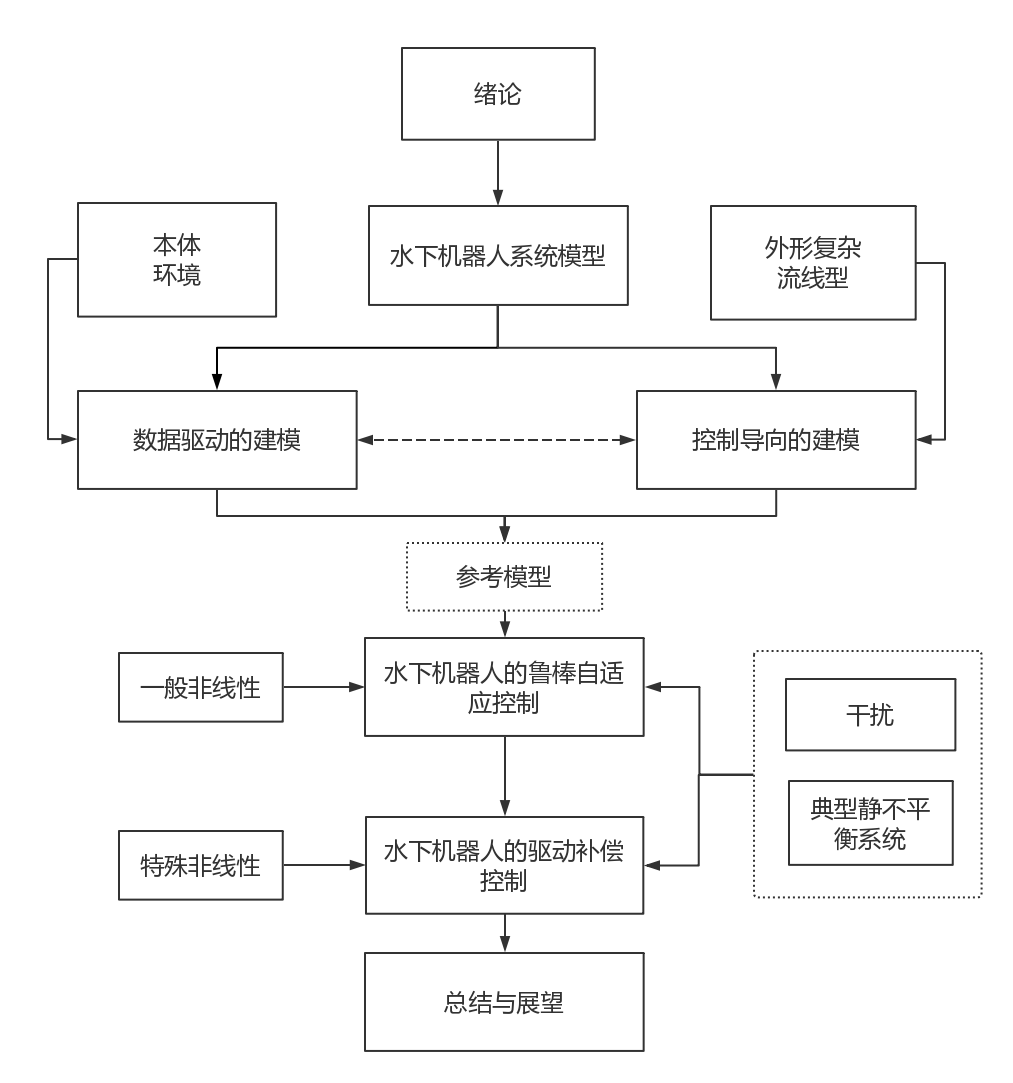
\includegraphics[width=14cm]{figure/chap1/diagram_2.png}
%\captionsetup{justification=centering}
\label{fig:chap1:F4}
\bicaption[fig:chap1:F4]{论文研究路线图}{论文研究路线图}{Fig.}{Diagram for this thesis}
\end{figure*}


\subsection{本文的研究路线图 }

% 水下机器人: ROV 外形复杂 AUV 流线型与鱼雷相类

% 系统建模 : 运动学动力学建模:驱动类型、推力分配与控制、 数据驱动建模:参数辨识、结构搜索、 环境建模:侧线原理、机器学习

% 控制应用的建模: 数值建模: 关键项:阻尼、附加质量   经验法、 数值计算法、 泰勒展开处理

% 控制 : 鲁棒性、 自适应性、 一般非线性、 特殊非线性、死区、延迟、阈值 现代补偿器、 基于Riccati方程的补偿器
本文的研究从水下机器人的系统分析展开,层层推进,进而实现研究目标。全文的研究路线如下所图\ref{fig:chap1:F4}所示:







\section{本章小结 }

本章中首先给出了水下机器人建模与非线性自适应控制的研究意义,着重对水下机器人的动力学建模与数据驱动的系统建模、鲁棒自适应控制及补偿优化进行了现状总结,提出围绕水下机器人的启发式建模与非线性问题问题的鲁棒自适应控制展开研究,重点放在水下机器人的数学模型搜索与系统辨识、水下机器人的控制导向的模型构建、鲁棒自适应控制以及驱动补偿控制上,并给出本文的研究路线图。
